\chapter{Modelos básicos en epidemiología}

\section{Tipos de modelos}

Los modelos discretos (principalmente SI, SIR y SIS) usan los estados Susceptible, Infectado y Recuperado. Los nombres suelen hacer referencia al flujo que se sigue para pasar entre los estados. Así, por ejemplo un modelo SI pasa de susceptible a infectado, uno SIR de susceptible a infectado y recuperado y SIS alterna entre susceptible e infectado.

En estos modelos se hacen dos suposiciones:
\begin{enumerate}
\item La población se mezcla de manera homogénea, es decir, todos los individuos tienen la misma probabilidad de contraer la enfermedad.
\item El total de la población es constante y lo denotaremos por $N$.
\end{enumerate}

En este capítulo estudiaremos los principales modelos epidemiológicos discretos y sus equivalentes continuos.

\section{Modelo SI}
El modelo SI es el modelo más simple de todos. Los individuos nacen siendo susceptibles a una enfermedad, y una vez infectados permanecen infectados el resto de su vida.
Un ejemplo de una enfermedad que pueda modelarse usando SI es el herpes.

Las siguientes ecuaciones describen el modelo SI discreto:

\begin{equation}
\label{eqn: SI}
\begin{aligned}
S_{n+1}=S_n\left( 1-\frac{\alpha\Delta t}{N}I_n\right) \\
I_{n+1}=I_n\left( 1+\frac{\alpha\Delta t}{N}S_n\right)
\end{aligned}
\end{equation}

donde $S_n$ indica el número de individuos susceptibles en el instante $t_n$, e $I_n$ hace referencia al número de individuos infectados en ese instante. $\Delta t$ es el tiempo transcurrido entre dos instantes $t_{n+1}-t_n$, y N es el tamaño total de la población, con condiciones iniciales $S_0>0$, $I_0>0$ y $S_0+I_0=N$.

En estas ecuaciones $\alpha$ es la tasa de contacto; es decir, el número medio de individuos con los que un infectado tiene suficiente contacto para contagiarlo en un intervalo de tiempo. Por tanto, $S_n$ representa el número de individuos susceptibles en el tiempo $n\Delta t$.

Pasaremos a imponer las suposiciones descritas anteriormente para estos modelos. En primer lugar, suponemos que la población se mezcla de manera homogénea de ahora en adelante. Para imponer la segunda suposición, la población total se mantiene constante, siendo trivial que se cumpla siempre, ya que sumando el sistema de ecuaciones el resultado es $N$ y asumimos que las soluciones son siempre positivas dado que las soluciones negativas no tienen sentido, ya que sería hablar de un número negativo de individuos, ya sean infectados, recuperados o susceptibles de contraer la enfermedad.

\begin{lemma}
$S_n$ es monótonamente decreciente e $I_n$ es monótonamente creciente.
\end{lemma}

\begin{proof}
$S_{n+1}$ es $S_n$ multiplicado por un valor menor que $1$, mientras que $I_{n+1}$ corresponde a $I_n$ multiplicado por un valor mayor que $1$.
\end{proof}

\begin{proposition}
Las soluciones de las ecuaciones \eqref{eqn: SI} son positivas si y solo si $\alpha\Delta t \leq 1$.
\end{proposition}

\begin{proof}
Supongamos que $I_n, S_n > 0$. Por la segunda ecuación del modelo \eqref{eqn: SI} es claro que $I_{n+1}>0$, pues $S_n>0$ y $1+\frac{\alpha\Delta t}{N}>0$.

Para la primera ecuación tenemos que $S_{n+1} > 0$ si y solo si
$$1-\frac{\alpha\Delta t}{N}I_n >0,$$

ya que $S_n$ es positivo por hipótesis. Esto equivale a $N>\alpha \Delta t I_n$, y puesto que $S_n+I_n=N$ se tiene:
$$N>\alpha\Delta t(N-S_n),$$
esto es
$$\alpha\Delta t S_n > (\alpha\Delta t -1) N.$$
Como $\alpha\Delta t S_n > 0$, tenemos entonces que la desigualdad se da para todo $n$ si y solo si:
$$\alpha\Delta t -1 \leq 0 \Leftrightarrow \alpha\Delta t \leq 1.$$
\end{proof}


Buscamos ahora ver cual es el comportamiento del sistema, calculando los puntos de equilibrio; esto es, las soluciones constantes en el tiempo, resolviendo:

$$
\begin{aligned}
S^*=S^*\left( 1-\frac{\alpha\Delta t}{N}I^*\right) \\
I^*=I^*\left( 1+\frac{\alpha\Delta t}{N}S^*\right) \\
S^*+I^*=N
\end{aligned}
$$

Los únicos puntos de equilibrio posibles son: $(S^*,I^*)=(0,N)$ y $(S^*,I^*)=(N,0)$. Puesto que las condiciones iniciales son positivas y como $S_n$ es monótonamente decreciente e $I_n$ es monótonamente creciente, así $S_{n+1}<S_n$ y $I_{n+1}>I_n$ para cualquier $n\in\mathbb{N}$, entonces debe converger a $(S^*,I^*)=(0,N)$, pues son sucesiones monótonas acotadas.

Expresando $\alpha$ como una tasa podemos obtener las ecuaciones diferenciales análogas de la siguiente manera. Considerando

$$\frac{S_{n+1} - S_n}{\Delta t} \approx S'(t),$$

El análogo continuo al sistema \eqref{eqn: SI} viene dado por:

\begin{equation}
\begin{aligned}
S'(t) = -\frac{\alpha}{N}SI \\
I'(t) = \frac{\alpha}{N}SI
\end{aligned}
\end{equation}

con condiciones iniciales $S(0)+I(0)=N$.

Calculamos los puntos de equilibrio de manera análoga al caso discreto, es decir, suponemos que las funciones son constantes y, resolviendo el sistema de ecuaciones, podemos comprobar que las soluciones convergen a $(S^*,I^*)=(0,N)$ y, por tanto, tienen el mismo comportamiento que el caso discreto.

Sustituyendo en el modelo $S=N-I$ obtenemos la ecuación diferencial logística

$$I'(t) = I\frac{\alpha}{N}(N-I).$$

Esta ecuación diferencial se puede resolver por separación de variables como sigue:

\begin{equation}
\begin{aligned}
I'(t)=\frac{\alpha}{N}I(N-I(t)) & \Leftrightarrow \int \frac{dI}{I(N-I)} = \int \frac{\alpha}{N} dt \\
& \Leftrightarrow \frac{1}{N}\int \left(\frac{1}{I}+\frac{1}{N-I}\right) dI = \frac{\alpha}{N}t+c \\
& \Leftrightarrow  \frac{1}{N}\log{\frac{I}{N-I}} = e^{\frac{\alpha}{N}t+c} \\
& \Leftrightarrow  \frac{I}{N-I} = e^ce^{\alpha t} \\
& \Leftrightarrow  I = e^ce^{\alpha t}(N-I) \\
& \Leftrightarrow  I(1+e^ce^{\alpha t}) = e^ce^{\alpha t}N \\
& \Leftrightarrow  I(t) = \frac{e^ce^{\alpha t}N}{1+e^ce^{\alpha t} }
\end{aligned}
\end{equation}

Usando el valor inicial $I(0)$ tenemos:

\begin{equation}
\begin{aligned}
I(0) = \frac{e^cN}{1+e^c} & \Leftrightarrow (1+e^c)I(0) = e^cN \\
& \Leftrightarrow e^c(N-I(0)) = I(0) \\
& \Leftrightarrow e^c = \frac{I(0)}{N-I(0)}
\end {aligned}
\end{equation}

luego la solución general es:

$$I(t) = \frac{I(0)e^{\alpha t}N}{(N-I(0))+I(0)e^{\alpha t}} = \frac{I(0)N}{(N-I(0))e^{-\alpha t}+I(0)}$$

Es claro que $I$ tiende monótonamente a $N$, luego tiene el mismo comportamiento que el modelo discreto.


\begin{figure}
\begin{center}
\caption{Gráfica del modelo SI discreto, en una población total de $100$ individuos, con valores iniciales $S_0=99, I_0 = 1, \alpha = 0.1, T_0 = 0, T = 100$.}
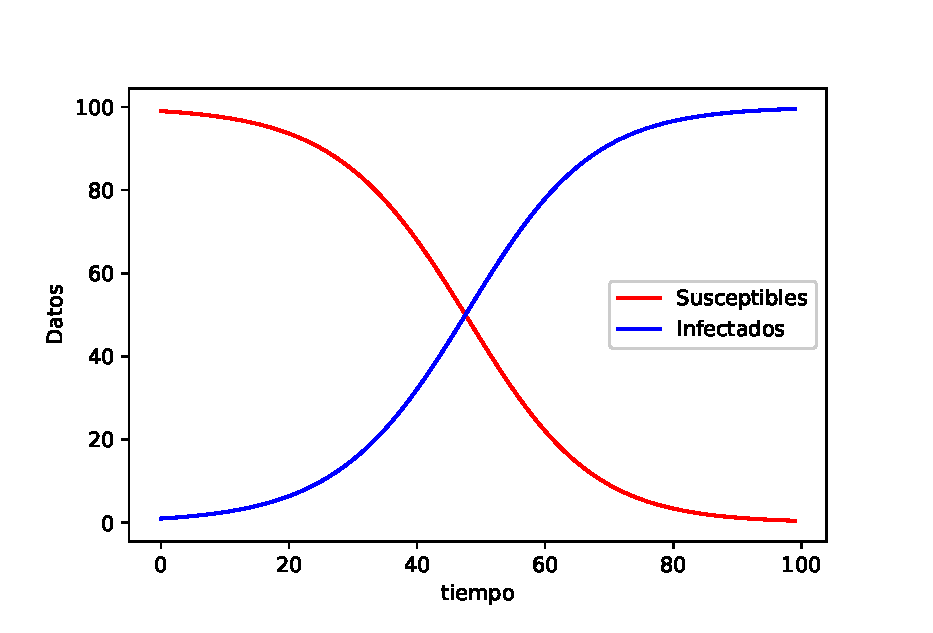
\includegraphics[scale=1]{graficaSI}
\end{center}
\end{figure}

En la figura \ref{fig: SI_IsobreS}, se representa el número de individuos infectados en función del númeor de susceptibles se aprecia una relación lineal pero inversamente proporcional, donde al subir el número de infectados baja el de susceptibles y al contrario.

\begin{figure}
\begin{center}
\caption{Gráfica del modelo SI, representando el número de infectados según el número de individuos susceptibles, en una población total de $100$ individuos, con valores iniciales $S_0=99, I_0 = 1, \alpha = 0.1, T_0 = 0, T = 100$.}
\label{fig: SI_IsobreS}
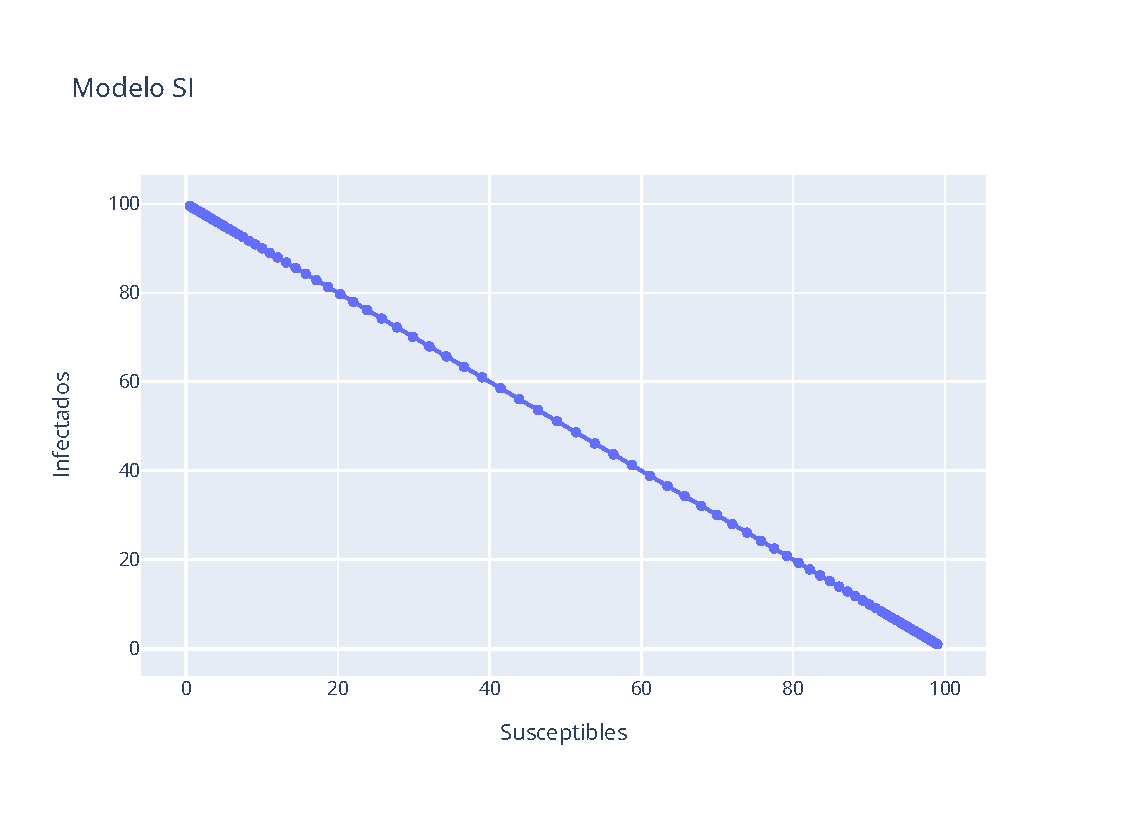
\includegraphics[scale=0.7]{SI_IsobreS}
\end{center}
\end{figure}

\section{Modelo SIR}
El modelo SIR comienza como el SI, pero tras infectarse los individuos pasan a un estado Recuperado, en el cual no pueden volver a infectarse ni infectar a otros.
Un ejemplo de este tipo de enfermedad es la varicela. 

El modelo es el siguiente:

\begin{equation}
\label{eqn: SIR_modelo}
\begin{aligned}
S_{n+1} = & S_n \left(1-\frac{\alpha\Delta t}{N} I_n \right) \\
I_{n+1} = & I_n \left( 1-\gamma \Delta t + \frac{\alpha\Delta t}{N} S_n \right) \\
R_{n+1} = & R_n + \gamma \Delta t I_n
\end{aligned}
\end{equation}

con condiciones iniciales $S_0>0$, $I_0>0$, $R_0\geq 0$, satisfaciendo $S_0+I_0+R_0=N$.

En estas ecuaciones, de nuevo tenemos que $\alpha$ es la tasa de contacto, esto es, el número medio de individuos con los que un infectado tiene suficiente contacto para contagiarlo en un intervalo de tiempo, y $\gamma$ es la probabilidad de que un infectado pase a recuperado/retirado/aislado/fallecido en un intervalo de tiempo, con $\alpha >0$ y $\gamma >0$.

Se supone que la población permanece constante, esto es: $S_n+I_n+R_n=N$.

\begin{proposition}
Las soluciones a este sistema discreto son positivas para cualquier valor de las condiciones iniciales si, y solo si:
$$\max{\big\{\gamma\Delta t, \alpha\Delta t\big\} } \leq 1$$

o equivalentemente:

$$\min{\bigg\{ \frac{1}{\gamma}, \frac{1}{\alpha} \bigg\} } \geq \Delta t$$

\end{proposition}

\begin{lemma}
$S_n$ es estrictamente decreciente y $R_n$ es estrictamentre creciente.
\end{lemma}

\begin{proof}

Sea $S_\infty=\lim_{n\rightarrow\infty} S_n\geq 0$, cuyo límite existe, pues es una sucesión estrictamente decreciente y acotada inferiormente por $0$.

Estudiamos las condiciones iniciales. Si $S_0\leq \frac{\gamma N}{\alpha}$, o, equivalentemente, $\mathcal{R}_{SIR}˘\leq 1$ entonces $I_1\leq I_0$ y, como $S_n$ es estrictamente decreciente, tenemos que $I_{n+1}\leq I_n$, es decir, no hay epidemia, ya que la velocidad de propagación no es lo bastante alta.

En otro caso, tenemos $S_0> \frac{\gamma N}{\alpha}$, entonces $I_1>I_0$. Debe ocurrir que $S_\infty <\frac{N\gamma}{\alpha}$, pues si no fuera así, tendríamos que $I_n$ crece hacia un equilibrio, $I_\infty$, lo que implica que $R_n$ se aproxima a infinito cuando $n\rightarrow\infty$, lo que no es posible, pues el total de la población es constante. Así, el número de infectados finalmente comienza a decrecer y se aproxima a $0$.
\end{proof}

\textcolor{red}{ el Lema 1 de \cite{allenDiscretetimeSISIR1994} dice que $S_\infty>0$. He estado mirando lo del lío con el límite de $S_n$, pero no he conseguido aclararme. Al hacerlo yo me sale que va a 0, pero el artículo original tiene este lema donde dice que el límite es mayor que 0 y no veo exactamente qué me estoy saltando en el razonamiento}

\begin{proof}
Comenzamos probando una de las implicaciones, suponiendo que $\max{\big\{\gamma\Delta t, \alpha\Delta t\big\} } \leq 1$.

Por hipótesis inicial, tenemos que $S_0, I_0, R_0>0$ y $S_0+I_0+R_0=N$, luego es suficiente comprobar que:
$$1-\frac{\alpha \Delta t}{N}I_0>0.$$
Lo cual es evidente, pues $\frac{I_n}{N}<1$ por hipótesis del modelo y $\alpha \Delta t<1$.

Por un razonamiento análogo, tenemos que $$1-\gamma \Delta t+\frac{\alpha\Delta t}{N}S_0 > 0.$$
Y finalmente $$R_0+\gamma\Delta t I_0>0$$ pues $\gamma>0$ y $\Delta t <0$.

Aplicando un razonamiento por inducción, suponiéndolo para $n$ se puede demostrar que $S_{n+1}, I_{n+1}, R_{n+1}$ son siempre positivas.

Para probar el recíproco basta probar que ambas cantidades son menores o iguales a $1$. Comenzamos trabajando en la primera ecuación \eqref{eqn: SIR_modelo}.
% suponemos la positividad para $n$ y probándola para $n+1$:

$$S_{n+1}=S_n\left(1-\frac{\alpha\Delta t}{N}I_n\right)$$
Por hipótesis $S_n>0$, entonces basta ver que $1-\frac{\alpha\Delta t}{N}I_n>0$. Usamos de nuevo que $I_n \leq N$ luego:
$$0<1-\frac{\alpha\Delta t}{N}I_n \leq 1-\alpha\Delta t,$$
y por tanto:
$$\alpha\Delta t  \leq 1.$$

En la segunda ecuación, como sabemos que $S_n$ es estrictamente decreciente, pues es una sucesión de la forma $S_{n+1}=\beta S_n$ con $\beta < 1$, entonces es cada vez más pequeño y el factor
$\frac{\alpha \Delta t}{N}S_n$ tiende a cero. \textcolor{red}{Aqui es donde uso que Sn tiende a 0, pero segun el articulo esto no es verdad}

Luego, despejando tenemos $\gamma\Delta t \leq 1$.

De la última ecuación no sacamos ninguna condición más, pues su solución es siempre positiva por definición de $\gamma$ y $\Delta t$.

\end{proof}

Por tanto, a partir del resultado anterior podemos deducir que el intervalo de tiempo, $\Delta t$, debe ser menor que el tiempo medio requerido para contagiar a oro individuo susceptible, $\alpha$, y menor que el período medio infeccioso, $\gamma$.
% Con contacto exitoso asumo que se refiere al tiempo necesario para infectar a un individuo. Sí es esto confirmado por la profe


El comportamiento global del sistema es fácil de ver. Definimos la tasa reproductiva como la constante 
$$\mathcal{R}_{SIR}=\frac{S_0 \alpha}{N\gamma }.$$

El valor de $\mathcal{R}_{SIR}$ determina el comportamiento global del modelo.

En otros trabajos como \cite{demongeotSIEpidemicModel} esta tasa reproductiva se llama tasa de transmisión media.

Además, sabemos por el Lema 1 de \cite{allenDiscretetimeSISIR1994} que $S_\infty>0$.
El modelo continuo correspondiente al modelo SIR se comporta de la misma forma que el modelo discreto, y viene expresado por:

\begin{equation}
\label{eqn: modelo_SIR_continuo}
\begin{aligned}
S'(t) = & -\dfrac{\alpha}{N}SI \\
I'(t) = & I\left(\dfrac{\alpha}{N}S-\gamma \right) \\
R'(t) = & R+\gamma I
\end{aligned}
\end{equation}

donde $S(0)+I(0)+R(0)=N$. La tasa reproductiva en este caso se define como
$$\mathcal{R}_{SIR}=\frac{S(0)\alpha }{N\gamma },$$
y si como hemos visto $\mathcal{R}_{SIR}\leq 1$  se dice que no hay epidemia, pero en cambio, si es mayor, se dice que sí la hay.

\begin{figure}
\begin{center}
\caption{Gráfica del modelo SIR, en una población total de $100$ individuos, con valores iniciales $S_0=99, I_0 = 1, R_0 = 0, \alpha = 0.1, \gamma = 0.01 T_0 = 0, T = 300$.}
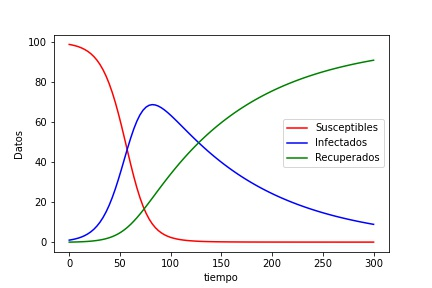
\includegraphics[scale=1]{graficaSIR}
\end{center}
\end{figure}

En la figura \ref{fig: SIR_IsobreS} se representan el número de infectados en función de los individuos susceptibles. En este modelo, al contrario de lo que ocurría en el modelo SI no son inversamente proporcionales. Vemos que primero los infectados crecen al descender el número de individuos susceptibles, esto es porque las personas susceptibles se infectan, pero después aunque los individuos susceptibles sigan disminuyendo los infectados bajan, esto es debido a que los individuos previamente infectados se están recuperando.

\begin{figure}
\begin{center}
\caption{Gráfica del modelo SI, representando el número de infectados según el número de individuos susceptibles, en una población total de $100$ individuos, con valores iniciales $S_0=99, I_0 = 1, \alpha = 0.1, \gamma=0.01, T_0 = 0, T = 300$.}
\label{fig: SIR_IsobreS}
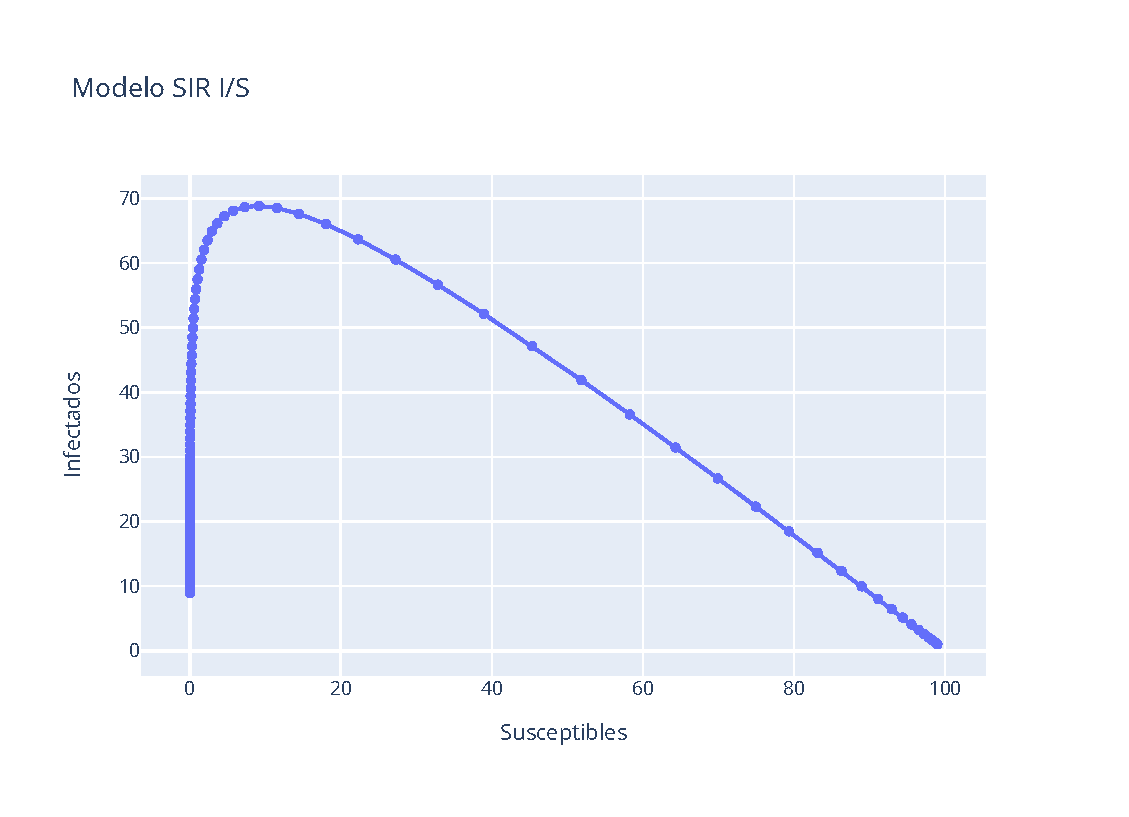
\includegraphics[scale=0.7]{SIR_IsobreS}
\end{center}
\end{figure}

Estudiamos ahora la figura \ref{fig: SIR_RsobreS}, en la que se muestra como varían los individuos recuperados en función de los susceptibles.

A medida que los individuos susceptibles decrecen los recuperados aumentan, pero no lo hacen de forma lineal. Esto se debe a que los individuos susceptibles primero deben infectarse y luego recuperarse, y, como ya hemos visto en la figura \ref{fig: SIR_IsobreS} los infectados bajan muy rápidamente cuando las personas susceptibles son pocas, por ello los recuperados también crecen rápidamente a menor número de individuos susceptibles.

\begin{figure}
\begin{center}
\caption{Gráfica del modelo SIR discreto, representando el número de recuperados según el número de individuos susceptibles, en una población total de $100$ individuos, con valores iniciales $S_0=99, I_0 = 1, \alpha = 0.1, \gamma=0.01, T_0 = 0, T = 300$.}
\label{fig: SIR_RsobreS}
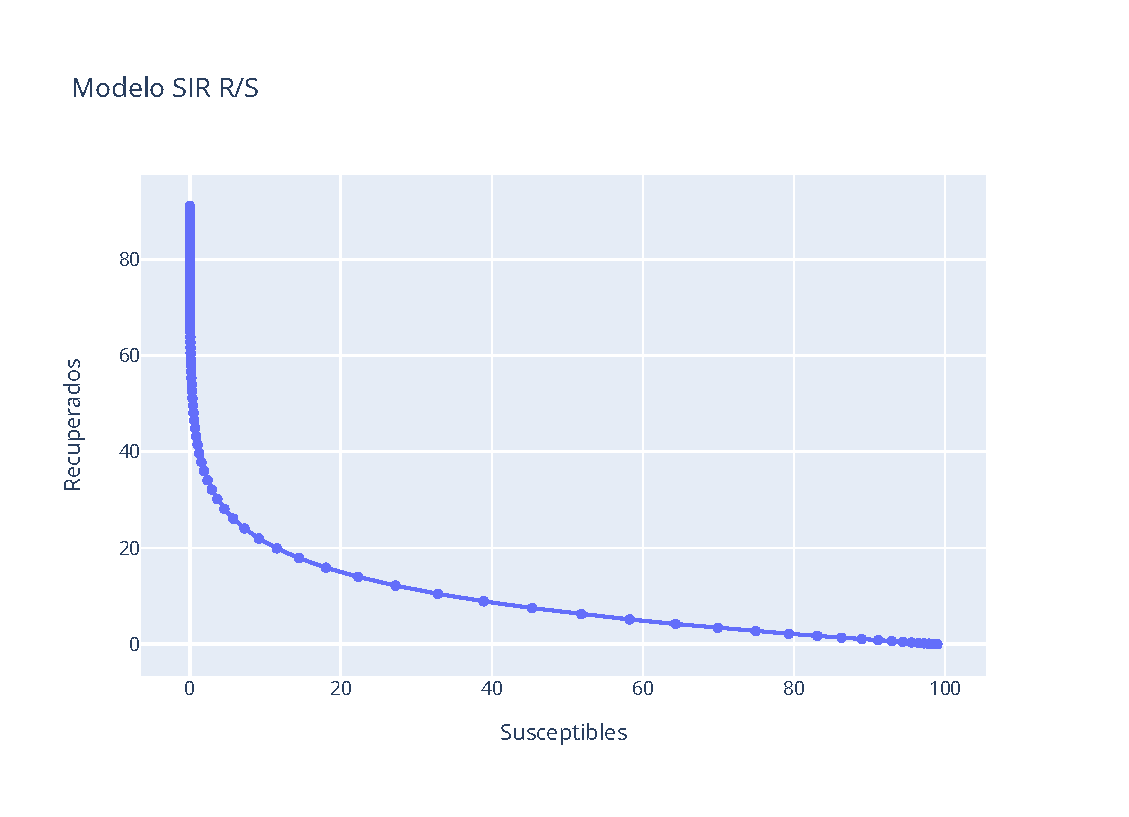
\includegraphics[scale=0.7]{SIR_RsobreS}
\end{center}
\end{figure}

Finalmente, en la figura \ref{fig: SIR_RsobreI} se muestran los individuos recuperados en función de los infectados.

Cabe destacar que para cada valor de los infectados hay dos valores de recuperados, esto se debe a que al comienzo, cuando los infectados están creciendo hay pocos recuperados, después los recuperados aumentan y los infectados decrecen. Es decir, para cada valor de infectados hay dos de recuperados, el primero cuando los infectados están creciendo y hay pocos recuperados y después cuando los infectados decrecen y hay muchos recuperados . Otra cosa a tener en cuenta es la distancia entre las marcas en la curva. Cada marca indica la medida del número de infectados y recuperados en un mismo tiempo $t$.

Al comenzar el número de recuperados es bajo y crece despacio a medida que aumentan los infectados. Llega un punto máximo del número de infectados, en el que se produce la curva, y cuando los infectados comienzan a descrecer los recuperados aumentan rápidamente, lo que se puede ver por la distancia más corta que hay entre las marcas de la curva.

\begin{figure}
\begin{center}

\caption{Gráfica del modelo SI discreto, representando el número de recuperados según el número de individuos infectados, en una población total de $100$ individuos, con valores iniciales $S_0=99, I_0 = 1, \alpha = 0.1, \gamma=0.01, T_0 = 0, T = 300$.}
\label{fig: SIR_RsobreI}
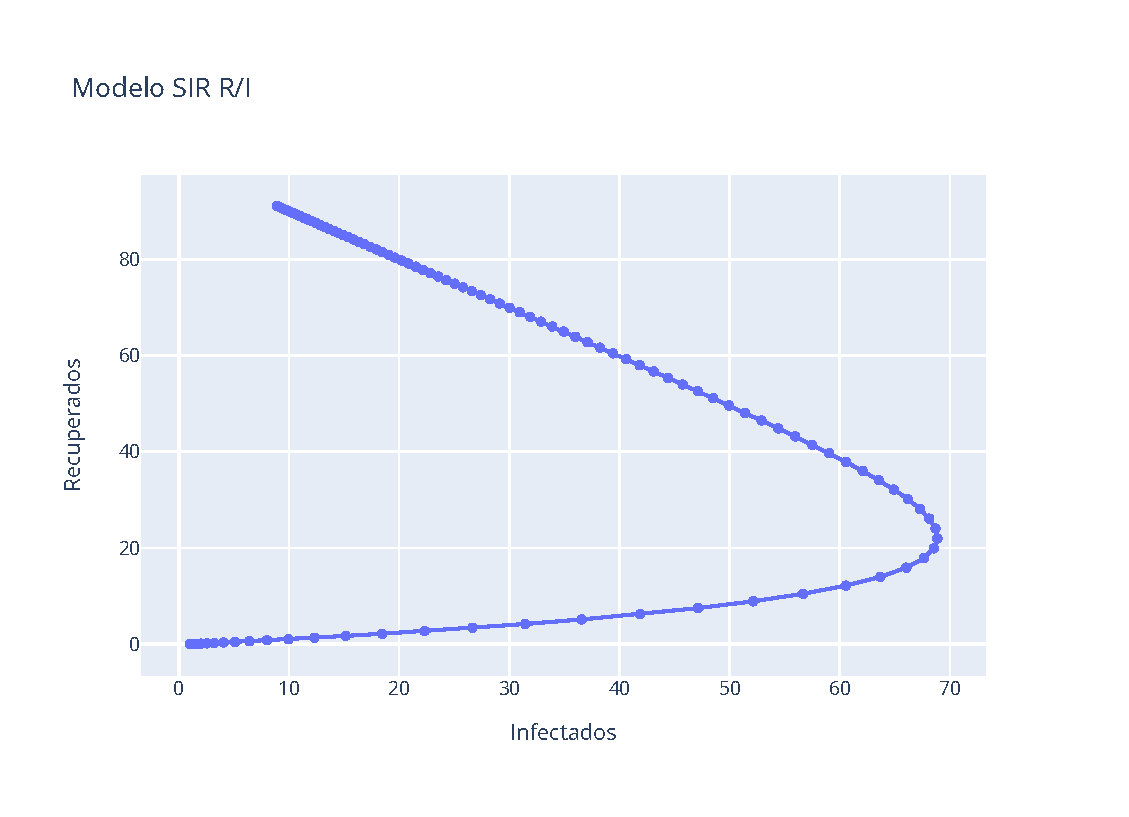
\includegraphics[scale=0.7]{SIR_RsobreI}
\end{center}
\end{figure}


\section{Modelo SIS}
El modelo SIS es similar al SI, con la salvedad de que los individuos son susceptibles de múltiples reinfecciones.
Por ejemplo, los resfriados pueden modelarse usando SIS.

El modelo es una perturbación del modelo SI descrito anteriormente. Se define de la siguiente forma:

\begin{equation}
\label{eqn: modelo_SIS}
\begin{aligned}
S_{n+1} = S_n \left(1-\frac{\alpha\Delta t}{N} I_n \right) + \gamma \Delta t I_n \\
I_{n+1} = I_n \left( 1-\gamma \Delta t + \frac{\alpha\Delta t}{N} S_n \right)
\end{aligned}
\end{equation}

con condiciones iniciales positivas $S_0>0$, $I_0>0$ cumpliendo $S_0+I_0=N$. Por lo tanto, el tamaño de la población es constante.

En estas ecuaciones, $\alpha$ de nuevo representa la tasa de contacto, esto es, el número medio de individuos con los que un infectado tiene suficiente contacto para contagiarlo en un intervalo de tiempo, y $\gamma$ es la probabilidad de que un infectado pase a recuperado/retirado/aislado/fallecido en un intervalo de tiempo, donde se cumple $\alpha >0$ y $\gamma >0$.

\begin{proposition}
Las soluciones de \eqref{eqn: modelo_SIS} siempre son positivas si, y solo si:

$$\gamma \Delta t \leq 1 $$ y $$\alpha\Delta t< \left( 1+\sqrt{\gamma \Delta t} \right)^2$$

\end{proposition}
\begin{proof}
Sea $I_0=\epsilon$ y $S_0=N-\epsilon$, entonces por la definición del modelo tenemos:
\begin{equation}
\begin{aligned}
I_1 & =\epsilon\left(1-\gamma\Delta t+\alpha\Delta t\frac{N-\epsilon}{N}\right) \\
& = -\frac{\alpha\Delta t \epsilon^2}{N} + \epsilon(1-\gamma\Delta t+\alpha\Delta t ) \\
& = p(\epsilon) \\
\end{aligned}
\end{equation}

Luego tenemos que ver cuándo la parábola satisface $0<p(\epsilon)<N$ para $0<\epsilon<N$.

Notemos que $p(0)=0$ y $p(N)=N(1-\gamma\Delta t).$

Sea $(\epsilon^*, p^*)$ el vértice de la parábola, entonces 
$$(\epsilon^*, p^*) = \left(\frac{N(1-\gamma\Delta t+\alpha\Delta t)}{2\alpha\Delta t}, \frac{N(1-\gamma\Delta t+\alpha\Delta t)^2}{4\alpha\Delta t}\right)$$

Por tanto, $0<p(\epsilon )<N$ para $0<\epsilon <N$ si y solo si:

$$\gamma\Delta t \leq 1,$$

y por tanto, o bien $\epsilon^* \geq N$, que es equivalente a $\alpha\Delta t \leq 1-\gamma\Delta t$. bien $\epsilon^*<N \text{  y  } p^*<N$, lo que requiere que $\alpha\Delta t > 1-\gamma\Delta t$ y $(1-\gamma\Delta t+\alpha\Delta t)^2<4\alpha\Delta t$. Estas desigualdades se dan si y solo si:

$$1-\gamma\Delta t < \alpha \Delta t < \left( 1+\sqrt{\gamma \Delta t} \right)^2.$$

\end{proof}

En el modelo SIS, la tasa reproductiva se define como 
$$\mathcal{R}_{SIS}=\frac{\alpha}{\gamma}.$$


\begin{lemma}
Si $\mathcal{R}_{SIS}\leq 1$ entonces se tiene que $I_{n+1} < I_n$, ya que $0<S_n<N$ y las soluciones son positivas. En este caso es fácil ver que el límite, al ser una sucesión monótona decreciente y acotada inferiormente, es $(S^*,I^*)=(N,0)$.

Si $\mathcal{R}_{SIS}>1$ las soluciones convergen si se cumple la condición$\alpha \Delta t \leq 2+\gamma \Delta t$
\end{lemma}

\begin{proof}
Supongamos que $S^*<N$, entonces existen $n_1, \epsilon$ tales que para todo $n \geq n_1$:
$$S_n<S^*+\epsilon < N$$
y usando las ecuaciones \eqref{eqn: modelo_SIS}
\begin{equation}
\begin{aligned}
I_{n+1}  & \leq I_n \left( 1-\gamma \Delta t + \frac{\alpha\Delta t}{N} S_n \right) \\
& \leq I_n \left( 1-\gamma \Delta t + \alpha\Delta t \right)
& \leq I_n \rho 
\end{aligned}
\end{equation}


donde hemos denotado $\rho = 1-\gamma \Delta t + \alpha\Delta t$.

Como $\rho < 1$ tendríamos que $I^*=0$, lo que contradice que $S^*<N$.

Si $\mathcal{R}_{SIS}>1$ realizando la sustitución $S_n=N-I_n$ y el cambio

$$x_n=\frac{\alpha \Delta t I_n}{N(1+\alpha \Delta t - \gamma \Delta t)}$$

tenemos:

\begin{equation}
\begin{aligned}
\alpha\Delta t I_n = x_nN(1+\alpha\Delta t-\gamma\Delta t) \Leftrightarrow \\
I_n = x_n\frac{N(1+\alpha\Delta t - \gamma\Delta t)}{\alpha\Delta t}
\end{aligned}
\end{equation}

entonces sustituyendo en la ecuación \eqref{eqn: modelo_SIS}:

\begin{equation}
\begin{aligned}
x_{n+1}\frac{N(1-\alpha\Delta t-\gamma\Delta t)}{\alpha \Delta t} = x_n\frac{N(1+\alpha\Delta t-\gamma \Delta t)}{\alpha\Delta t}\left( 1-\gamma\Delta t+\frac{\alpha\Delta t}{N}\left(N-x_n\frac{N(1+\alpha\Delta t-\gamma\Delta t)}{\alpha\Delta t}\right) \right)
\end{aligned}
\end{equation}

Despejando de esta expresión:

\begin{equation}
\begin{aligned}
x_{n+1} & = x_n\left( 1-\gamma\Delta t+\frac{\alpha\Delta t}{N}N-\frac{\alpha\Delta t}{N}x_n\frac{N(1+\alpha\Delta t -\gamma \Delta t)}{\alpha\Delta t} \right) \\
& = x_n(1-\gamma\Delta t + \alpha\Delta t -x_n(1+\alpha\Delta t -\gamma\Delta t)) \\
& = x_n((1-\gamma\Delta t+\alpha\Delta t)(1-x_n))
\end{aligned}
\end{equation}

luego obtenemos la ecuación logística con parámetro $\mu = 1+\alpha\Delta t -\gamma \Delta t$

$$x_{n+1} = (1+\alpha \Delta t - \gamma \Delta t)x_n(1-x_n).$$

En el modelo SIS la restricción necesaria para garantizar soluciones positivas no es suficiente para asegurar la convergencia. En este caso a dicha restricción hay que añadir la condición $\alpha \Delta t \leq 2+\gamma \Delta t$, restricción del parámetro de la ecuación logística para la convergencia.

\end{proof}


\begin{figure}
\begin{center}
\caption{Gráfica del modelo SIS, en una población total de $100$ individuos, con valores iniciales $S_0=95, I_0 = 5, \alpha = 0.1, \gamma=0.01, T_0 = 0, T = 150$.}
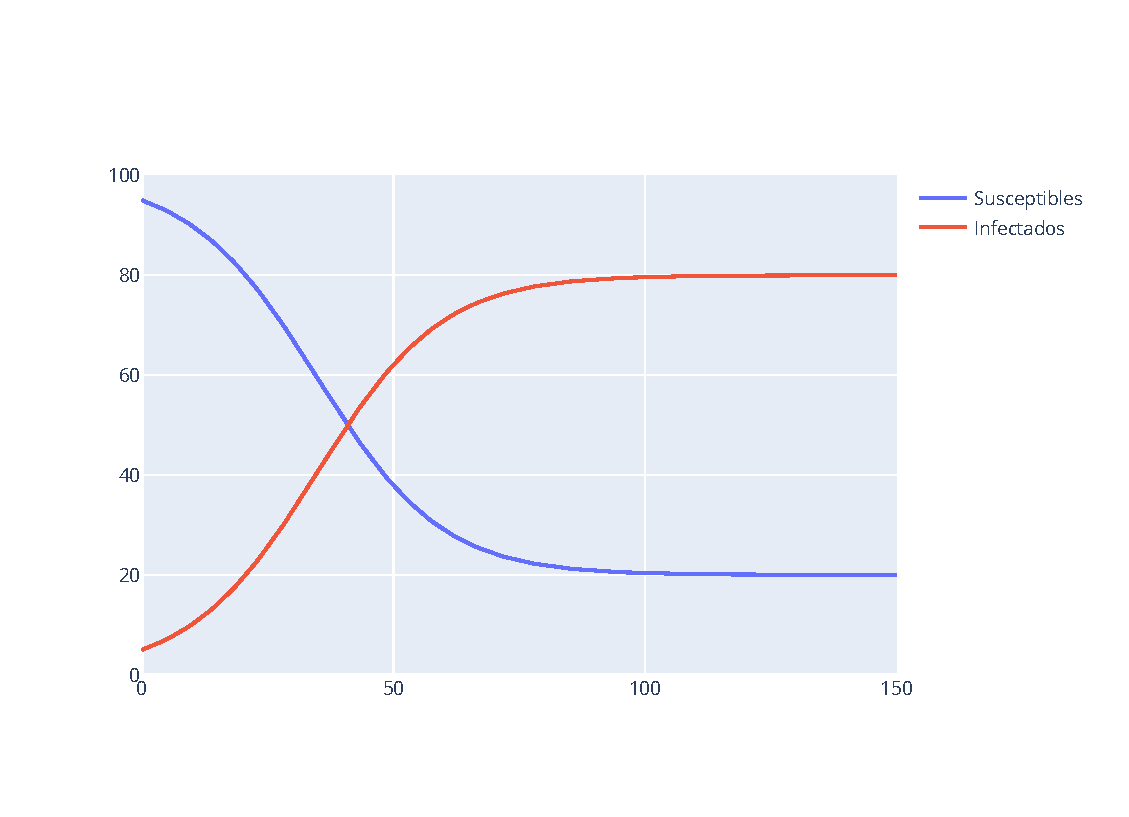
\includegraphics[scale=0.7]{SIS_modelo}
\end{center}
\end{figure}

En la figura \eqref{fig: SIS_IsobreS} se representa el número de infectados en función del número de individuos susceptibles. Se puede ver que son inversamente proporcionales, es decir, a mayor número de infectados menos individuos susceptibles hay y al revés.

Cabe destacar el parecido de esta gráfica con su análoga del modelo SI \eqref{fig: SI_IsobreS}.

\begin{figure}
\begin{center}
\caption{Gráfica del modelo SIS discreto, representando el número de infectados según el número de individuos susceptibles, en una población total de $100$ individuos, con valores iniciales $S_0=95, I_0 = 5, \alpha = 0.1, \gamma=0.01, T_0 = 0, T = 200$.}
\label{fig: SIS_IsobreS}
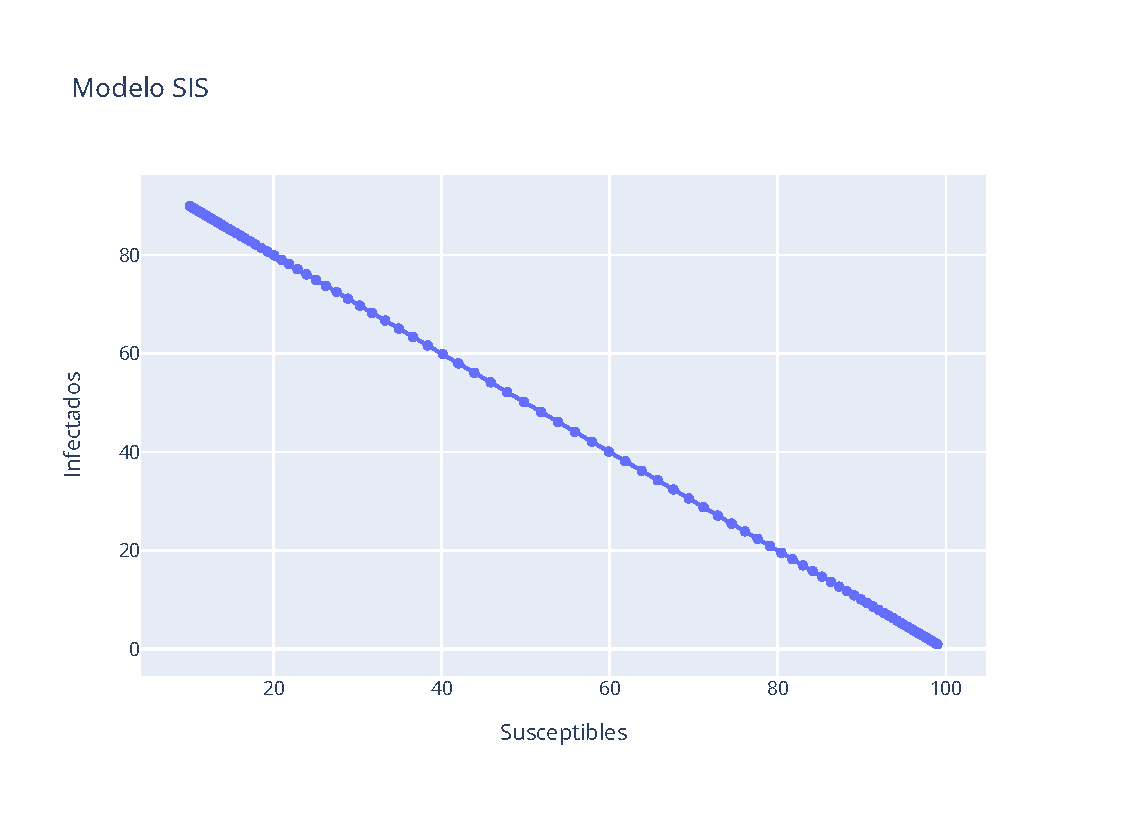
\includegraphics[scale=0.7]{SIS_IsobreS}
\end{center}
\end{figure}







\section{Análisis de los parámetros de los modelos}

\subsection{Introducción}

Estimar la tasa de transmisión media es uno de los aspectos más cruciales en epidemiología. Esta tasa condiciona la fase de la epidemia e incluso si va a extinguirse. Es combinación de tres factores:

\begin{enumerate}
\item Coeficiente de virulencia: Relacionado con el agente infeccioso.
\item Coeficiente de susceptibilidad: Relacionado con el anfitrión.
\item Número de contactos por unidad de tiempo entre individuos.
\end{enumerate}

Los dos primeros factores se tienen en cuenta a la vez en la probabilidad de transmisión.

Todos los factores pueden cambiar con el tiempo. El primero, debido a mutaciones del virus y los dos últimos por medidas de contención. Por tanto, observar el decrecimiento de la transmisión media en una enfermedad es una buena forma de comprobar la efectividad de las medidas de contención.

En el artículo \cite{demongeotSIEpidemicModel} se presenta un modelo SI modificado con el objetivo de compararlo con los datos obtenidos en la pandemia de la COVID-19 hasta el momento, y así tratar de predecir su comportamiento en el futuro.

El modelo SI continuo considerado es el siguiente:

\begin{equation}
\label{eqn: SI_cont}
\begin{aligned}
S'(t) = & -\tau (t)S(t)I(t) \\
I'(t) = & \tau (t)S(t)I(t) -vI(t)
\end{aligned}
\end{equation}

donde $S(t)$ es el número de individuos susceptibles , $I(t)$ el número de individuos infectados en el tiempo $t$ y $\tau (t)$ la tasa de transmisión, que combina el número de contactos por unidad de tiempo y la probabilidad de transmisión. Observemos que $\tau (t)$ se considera variable respecto al tiempo, al contrario que en el caso SI clásico estudiado antes. Además, notemos que $v$ es una constante, donde $1/v$ es la duración media del período de infección, y $vI(t)$ el flujo de individuos recuperados o fallecidos. %vI(t) es el flujo de recuperados o muertos porque ha mezclado el modelo SI y SIR; vI(t) serian los recuperados, pero se ahorra la ecuacion de la R

Se consideran las condiciones iniciales

$$S(t_0)=S_0>0, \: I(t_0)=I_0>0.$$

Ahora, consideramos que al final del período infeccioso nos han informado de una fracción del total de casos, en este caso la fracción la denotamos por $f\in (0,1]$. Sea $C_R(t)$ el número total acumulado de casos reportados. Entonces:

\begin{equation}
\label{eqn: acumulada}
C_R(t) = {C_R}_0 + vfC_I(t) \; \forall t \geq t_0
\end{equation}

donde $C_{R0}$ representa el número de casos reportados al inicio del estudio y 

$$C_I(t) = \int_{t_0}^t I(w) dw $$

siendo $C_I$ el número total de infectados acumulado.

Asumimos conocidos $S_0 > 0$, $1/v>0$, $f\in (0,1]$. Por tanto, queremos averiguar el número inicial de infectados $I_0$ y la tasa de transmisión $\tau (t)$.

\subsection{Aproximación de $I_0$ y $\tau (t_0)$}
Procedemos a intentar aproximar $I_0$ y $\tau (t_0)$:

Al comienzo de la pandemia podemos suponer que $S(t)$ y $\tau (t)$ son constantes e iguales a $S_0$ y $\tau_0 = \tau (t_0)$, respectivamente. Sustituyendo estos valores en la ecuación \eqref{eqn: SI_cont} obtenemos:

$$I'(t) = (\tau_0 S_0 -v) I(t).$$

Resolviendo la ecuación diferencial llegamos a:

$$I(t) = I_0\exp{((\tau_0 S_0-v)(t-t_0))}.$$

Sustituyendo en \eqref{eqn: acumulada}:

$$C_R(t) = {C_R}_0 + vfI_0\frac{\mathrm{e}^{(\tau_0 S_0 -v)(t-t_0)} -1}{\tau_0 S_0-v}.$$

De este modo, hemos obtenido un primer modelo para los casos acumulados al principio de la pandemia.

Reescribimos la ecuación anterior como:

\begin{equation}
\label{eqn: acumulada_modelo}
C_R(t) = \chi_1 \mathrm{e}^{\chi_2 t} -\chi_3.
\end{equation}

Estimamos $\chi_3$ usando los datos de la epidemia obtenidos, y el mejor ajuste para los datos se obtiene con $\chi_3=0$.

Ahora, usando \eqref{eqn: acumulada} y \eqref{eqn: acumulada_modelo} tenemos:

\begin{equation}
I_0=\frac{\chi_1\chi_2\mathrm{e}^{\chi_2 t_0}}{vf}
\end{equation}

Y, como sabemos que $\chi_2 = \tau_0 S_0-v$, entonces

\begin{equation}
\tau_0 = \frac{\chi_2+v}{S_0}.
\end{equation}

Si suponemos $\tau (t) = \tau_0$ constante, tenemos que el modelo queda:

\begin{equation}
\begin{aligned}
S'(t) = -\tau_0S(t)I(t) \\
I'(t) = \tau_0S(t)I(t) -vI(t)
\end{aligned}
\end{equation}

Usando la ecuación de $S(t)$ y resolviéndola obtenemos:

$$S(t) = S_0\exp{\left( -\tau_0 \int_{t_0}^t I(w) dw \right)} = S_0\exp{(-\tau_0 C_I(t))}$$

Ahora, sustituyendo esta expresión en la ecuación de $I(t)$ del modelo y usando $C_I'(t)=I(t)$:

$$I'(t) = S_0\exp{\left( -\tau_0 C_I(t)\right) }\tau_0 C_I'(t)-vI(t)$$

Finalmente, integrando entre $t_0$ y $t$ tenemos que:

$$I(t)=C_I'(t)=I_0+S_0(1-\exp{(-\tau_0 C_I(t)}))-vC_I(t)$$
 
Observamos entonces que el número total de infectados es monótono creciente, ya que $I(t)>0$ siempre por positividad de las soluciones y $C_I'(t)=I(t)>0$. Cabe destacar que esto no implica que el número de infectados sea monótono creciente.

\begin{theorem}
Sea $t>t_0$ fijo. El número de infectados acumulados es estrictamente creciente respecto a las siguiente cantidades:
\begin{itemize}
\item $I_0>0$: Número inicial de infectados
\item $S_0>0$: Número inicial de individuos susceptibles.
\item $\tau>0$: Tasa de transmisión
\item $1/v$: Tiempo medio de la infección.
\end{itemize}
\end{theorem}

\subsection{Fórmula teórica para $\tau (t)$}

Usando la ecuación del modelo inicial \eqref{eqn: SI_cont} obtenemos:
% La ecuacion de la S$

$$S(t) = S_0 \exp{\left( - \int_{t_0}^t \tau(w) I(w) dw \right) } $$ 

Ahora, sustituyendo en la ecuación \eqref{eqn: SI_cont}:
% La ecuacion de la I

$$I'(t) = S_0 \exp{\left( - \int_{t_0}^t \tau(w) I(w) dw \right) } \tau (t) I(t) -vI(t) $$

Integramos en ambos lados entre $t_0$ y $t$, luego:

$$ C_I'(t) = I_0 + S_0 \left( 1-\exp{\left(- \int_{t_0}^t \tau (w) I(w)dw \right)}\right) -vC_I(t)$$

Equivalentemente, por \eqref{eqn: acumulada}:

$$C_R'(t) = vf\left( I_0 + S_0 \left( 1-\exp{\left(- \frac{1}{vf}\int_{t_0}^t \tau (w ) I(w)dw \right)}\right)\right) +v{C_R}_0 -vC_R(t)$$

\textcolor{red}{TODO Esta cuenta no termina de salirme, pero tiene más o menos sentido}

Así, obtenemos el Teorema 3.1 de \cite{demongeotSIEpidemicModel}, que nos da la relación directa buscada.

\textcolor{blue}{He estado leyendo el resto del artículo, en el que habla de obtener una expresión explícita de $\tau (t)$ e $I_0$, pero para eso usan datos de China en específico y ajustes por ordenador, así que no tengo muy claro si merece la pena incluir esa parte ya que no tenemos los datos y por tanto sería fiarse un poco de lo que han hecho ellos}







